\documentclass[12pt, a4paper]{article}

% ~~~~~~~~~~ Preamble: Packages and Document Setup ~~~~~~~~~~
\usepackage[utf8]{inputenc}
\usepackage{graphicx}
\usepackage{amsmath}
\usepackage{geometry}
\usepackage{setspace}
\usepackage{booktabs} % For better table rules
\usepackage{caption}
\usepackage{subcaption} % For arranging figures
\usepackage{xcolor}   % For colors in tables and text
\usepackage{listings} % For code blocks
\usepackage{hyperref}
\usepackage[style=numeric, sorting=none, backend=biber]{biblatex}
\addbibresource{references.bib} % The .bib file you will create

% Page geometry
\geometry{
 a4paper,
 left=25mm,
 right=25mm,
 top=25mm,
 bottom=25mm,
}

% Hyperlink setup
\hypersetup{
    colorlinks=true,
    linkcolor=blue,
    citecolor=green,
    filecolor=magenta,      
    urlcolor=cyan,
    pdftitle={SPEI Computation and Visualization Pipeline},
    pdfpagemode=FullScreen,
}

% Spacing
\onehalfspacing

% Code listing style
\definecolor{codegreen}{rgb}{0,0.6,0}
\definecolor{codegray}{rgb}{0.5,0.5,0.5}
\definecolor{codepurple}{rgb}{0.58,0,0.82}
\definecolor{backcolour}{rgb}{0.95,0.95,0.92}

\lstdefinestyle{mystyle}{
    backgroundcolor=\color{backcolour},   
    commentstyle=\color{codegreen},
    keywordstyle=\color{magenta},
    numberstyle=\tiny\color{codegray},
    stringstyle=\color{codepurple},
    basicstyle=\ttfamily\footnotesize,
    breakatwhitespace=false,         
    breaklines=true,                 
    captionpos=b,                    
    keepspaces=true,                 
    numbers=left,                    
    numbersep=5pt,                  
    showspaces=false,                
    showstringspaces=false,
    showtabs=false,                  
    tabsize=2
}
\lstset{style=mystyle}


% ~~~~~~~~~~ Title and Author ~~~~~~~~~~
\title{\huge\textbf{SPEI Computation and Visualization Pipeline}}
\author{\large\textbf{Pushkin Mangla} \\ \normalsize{Department of Computer Science and Engineering, IIT Delhi}}
\date{}

% ~~~~~~~~~~ Document Begins ~~~~~~~~~~
\begin{document}

\maketitle
\tableofcontents
\newpage

\begin{abstract}
    \noindent This document presents a complete pipeline for calculating and visualizing the \textbf{SPEI (Standardized Precipitation Evapotranspiration Index)}, a tool for drought assessment. The methodology is built upon open-access geospatial datasets, including precipitation (\textbf{P}) data from \textbf{CHIRPS} and Potential Evapotranspiration (\textbf{PET}) data from \textbf{MODIS}. This work is contextualized within broader efforts to build digital public goods for climate resilience, such as the CORE Stack initiative \cite{seth2024core}.
    \newline\newline
    As a case study, this documentation details an analysis for the state of Madhya Pradesh, India, for the years 2004-2023. The primary objective is to assess drought conditions at monthly, seasonal, and annual scales using \textbf{SPEI-1}, \textbf{SPEI-3}, and \textbf{SPEI-12}, respectively.
\end{abstract}

\section{Data Sources}

\begin{table}[h!]
    \centering
    \caption{Primary datasets used for SPEI calculation.}
    \begin{tabular}{p{6cm} p{6cm}}
        \toprule
        \textbf{Dataset Description} & \textbf{Link} \\
        \midrule
        \textbf{CHIRPS Daily v2.0} \newline Precipitation data ($0.05^{\circ}$ resolution), 1981-present & \href{https://developers.google.com/earth-engine/datasets/catalog/UCSB-CHG_CHIRPS_DAILY}{CHIRPS - Earth Engine} \\
        \addlinespace
        \textbf{MODIS MOD16A2GF v6.1} \newline 8-day Potential Evapotranspiration (PET) from MODIS & \href{https://developers.google.com/earth-engine/datasets/catalog/MODIS_061_MOD16A2GF}{MODIS PET - Earth Engine} \\
        \addlinespace
        \textbf{FAO GAUL} \newline Administrative boundaries of Indian states & \href{https://developers.google.com/earth-engine/datasets/catalog/FAO_GAUL_2015_level1}{FAO/GAUL/2015 - Earth Engine} \\
        \bottomrule
    \end{tabular}
\end{table}

\section{Study Area}
The area of interest is \textbf{Madhya Pradesh}, extracted using the FAO/GAUL boundaries dataset by filtering for ADM0\_NAME = India and ADM1\_NAME = Madhya Pradesh. All analysis and exports are spatially clipped to this region.

\section{Methodology}

\subsection{Step 1: Computation of Monthly P - PET}
For each month from January, 2004 - December, 2023, the climatic water balance for each pixel in Madhya Pradesh was calculated as:
\[ D_i = P_i - PET_i \]
where $D_i$ is the water balance (P-PET) for month $i$.

\begin{itemize}
    \item CHIRPS data was aggregated daily into monthly sums for Precipitation ($P_i$).
    \item MODIS PET (8-day composites) was also summed for each month and rescaled using a factor of 0.1 to get Potential Evapotranspiration ($PET_i$).
    \item The monthly difference ($D_i$) was computed in Google Earth Engine and exported as GeoTIFF files.
\end{itemize}

\textit{\{During this process, as the resolution for CHIRPS P data is $0.05^{\circ}$ and MODIS PET is 500m, the MODIS PET resolution was resampled to $5.5km \approx 0.05^{\circ}$ to match. This was validated as acceptable using the Global Moran's I statistic.\}}

The code for the export of these 240 .tif images is available externally.

\begin{center}
    \textit{The GEE script can be found at: \href{https://github.com/Actuallyanonymous/spei-drought-analysis-pipeline/blob/main/scripts/01_gee_export_pp-et.py}{01\_gee\_export\_pp-et.py}}
\end{center}


\subsection{Step 2: SPEI Standardization in Python}
Once the monthly water balance (P-PET) rasters were generated, the time series for each pixel was standardized to compute the SPEI. This process transforms the raw water balance data into a standardized index where values represent deviations from a long-term average, making them comparable across different locations and times.

\subsubsection{Theoretical Background of SPEI Standardization}
The core of the SPEI calculation is to fit a probability distribution to the time series of the water balance data ($D_i$), and then transform the resulting cumulative probabilities to a standard normal distribution. This methodology is based on the work of Vicente-Serrano et al. (2010) \cite{vicente2010multiscalar} and further information is available from the SPEI Global Drought Monitor \cite{spei_csic}.

\begin{enumerate}
    \item \textbf{Aggregation at Different Timescales:} The water balance data is first aggregated at different time scales to calculate SPEI for different purposes. For example, to calculate SPEI-3 (seasonal drought), a 3-month moving average of the $D_i$ series is computed.
    \[ D^k_n = \sum_{i=0}^{k-1} D_{n-i} \]
    where $k$ is the timescale (e.g., 1, 3, or 12 months) and $n$ is the calculation month.

    \item \textbf{Fitting a Probability Distribution:} For each pixel, the time series of aggregated water balance values ($D^k$) is fitted to a probability distribution. While the original paper suggests a three-parameter log-logistic distribution, this pipeline uses the \textbf{Generalized Logistic (genlogistic)} distribution from SciPy, which is well-suited for modeling hydrological data that can be skewed. The Probability Density Function (PDF) is given by:
    \[ f(x) = \frac{c e^{-z}}{\sigma (1+e^{-z})^{c+1}} \quad \text{where} \quad z = \frac{x-\mu}{\sigma} \]
    Here, $\mu$ is the location parameter, $\sigma$ is the scale parameter, and $c$ is the shape parameter. These parameters are estimated from the data series for each pixel.

    \item \textbf{Calculating Cumulative Probability:} Using the fitted parameters, the cumulative distribution function (CDF) is used to calculate the probability of observing a given water balance value, $F(x)$.
    \[ F(x) = \left(1+e^{-z}\right)^{-c} \]

    \item \textbf{Standardization:} The final step is to transform the cumulative probability $F(x)$ into a standard normal variable (Z-score) with a mean of zero and a standard deviation of one. This Z-score is the SPEI value. This is achieved by using the inverse of the standard normal CDF, also known as the quantile function ($\Phi^{-1}$).
    \[ SPEI = \Phi^{-1}(F(x)) = \text{norm.ppf}(F(x)) \]
    The resulting SPEI values are standardized and can be interpreted as the number of standard deviations a given water balance value deviates from the long-term mean.
\end{enumerate}

\subsubsection{Implementation Process}
The theoretical steps above are implemented in Python as follows:
\begin{enumerate}
    \item Stack 240 monthly images using \texttt{rasterio}.
    \item Apply rolling sums over 1-month, 3-month, and 12-month windows.
    \item For each pixel's time series, fit the Generalized Logistic Distribution using \texttt{scipy.stats.genlogistic.fit}.
    \item Transform the resulting CDF values into a standard normal (Z-score) distribution using \texttt{scipy.stats.norm.ppf}.
\end{enumerate}

The Python code for this standardization is available externally.
\begin{center}
    \textit{The full script can be found at: \href{https://github.com/Actuallyanonymous/spei-drought-analysis-pipeline/blob/main/scripts/02_calculate_spei.py}{02\_calculate\_spei.py}}
\end{center}


\textbf{Output:}
\begin{itemize}
    \item \textbf{SPEI1\_001.tif to SPEI1\_240.tif:} Monthly SPEI-1 $\rightarrow$ 240 (12*20) images.
    \item \textbf{SPEI3\_YYYY\_MM.tif:} Seasonal SPEI-3 (March, June, Sept, Dec of each year) $\rightarrow$ 80 (4*20) images.
    \item \textbf{SPEI12\_YYYY\_tif:} Annual SPEI-12 (December only) $\rightarrow$ 20 (1*20) images.
\end{itemize}
\textbf{Total:} $240 + 80 + 20 = 340$ images for 20 years (17 for each year).

\subsection{Step 3: Upload to Google Earth Engine}
As the automation of uploading assets into GEE failed, only selected images were manually uploaded to visualize the results. For initial visualization, only a few images were uploaded on GEE. Each image was uploaded as an individual asset.

\subsection{Step 4: Visualization and Z-score Normalization}
All visualization was done in the Google Earth Engine Code Editor using the uploaded assets. We compared January/Seasonal/Annual values across years using a pixel-wise Z-score to identify anomalies:
\[ Z = \frac{(\text{SPEI value} - \text{mean of all years})}{\text{std deviation of all years}} \]
Here the mean and standard deviation were calculated for a window of 20 years (2004-2023). This window can remain fixed for further analysis. This method helped identify spatial drought anomalies in specific years.

The GEE script for this visualization is available externally.
\begin{center}
    \textit{The full script can be found at: \href{https://github.com/Actuallyanonymous/spei-drought-analysis-pipeline/blob/main/scripts/03_gee_visualize_spei.js}{03\_gee\_visualize\_spei.js}}
\end{center}

A diverse color palette was used to visualize the droughts clearly:
\begin{table}[h!]
    \centering
    \caption{Z-SPEI Visualization Palette}
    \begin{tabular}{llll}
        \toprule
        \textbf{Z-SPEI Range} & \textbf{Interpretation} & \textbf{Hex Code} & \textbf{Color Name (Approximate)} \\
        \midrule
        < -2 & Extreme Drought & \#8c2d04 & Dark Brown \\
        -2 to -1.5 & Severe Drought & \#d94801 & Reddish Orange \\
        -1.5 to -1 & Moderate Drought & \#f16913 & Orange \\
        -1 to -0.5 & Mild Drought & \#fdae6b & Light Orange/Peach \\
        -0.5 to 0 & Slightly Drier & \#fdd0a2 & Pale Peach/Sand \\
        $\approx$ 0 & Normal & \#f7f7f7 & Very Light Gray/Off-White \\
        0 to 0.5 & Slightly Wetter & \#d4e6f5 & Pale Blue \\
        0.5 to 1 & Mild Wetness & \#92c5de & Light Blue \\
        1 to 1.5 & Moderate Wetness & \#4393c3 & Medium Blue \\
        1.5 to 2 & Severe Wetness & \#2166ac & Deep Blue \\
        > 2 & Extremely Wet & \#053061 & Navy Blue/Very Dark Blue \\
        \bottomrule
    \end{tabular}
\end{table}

\subsection{Result Verification Example}
The multi-scalar nature of SPEI allows for a comprehensive analysis of drought events. The year \textbf{2015} serves as an excellent case study. The SPEI-1 for January 2015 (Figure \ref{fig:2015_results}a) indicates significant drought conditions at the beginning of the year.

However, the SPEI-3 for the monsoon season of July-September (Figure \ref{fig:2015_results}b) shows a period of near-normal or even slightly wet conditions. This can be attributed to monsoon rainfall temporarily alleviating the water deficit, coupled with lower PET during this period.

Despite the mid-year relief, the SPEI-12 for the entire calendar year (Figure \ref{fig:2015_results}c) reveals a severe to extreme drought, confirming that the annual water balance was overwhelmingly negative. This aligns with ground reports: on \textbf{Oct 26, 2015}, Madhya Pradesh officially declared a drought in 33,283 villages, affecting 4.4 million hectares and 4.8 million farmers, as documented by the South Asia Network on Dams, Rivers and People \cite{sandrp2015} and the Directorate of Pulses Development \cite{dpd2015}. This demonstrates the pipeline's ability to capture both short-term variations and the overarching annual drought severity.

\begin{figure}[h!]
    \centering
    \begin{subfigure}[b]{0.48\textwidth}
        \centering
        \includegraphics[width=\textwidth]{spei_jan_2015.png}
        \caption{SPEI-1 for January 2015, showing initial drought conditions.}
        \label{fig:2015_jan}
    \end{subfigure}
    \hfill
    \begin{subfigure}[b]{0.48\textwidth}
        \centering
        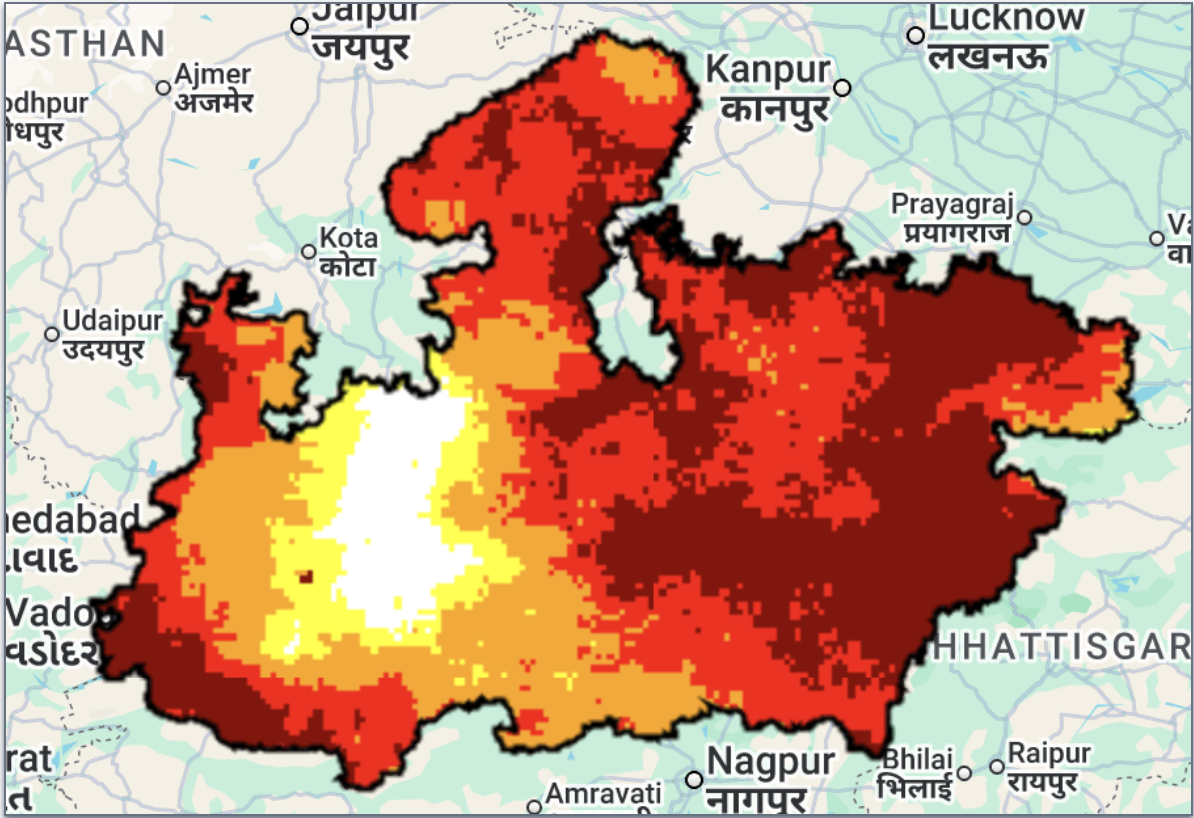
\includegraphics[width=\textwidth]{spei_jul-sep_2015.png}
        \caption{SPEI-3 for July-September 2015, showing temporary relief.}
        \label{fig:2015_season3}
    \end{subfigure}
    
    \vspace{1cm} % Add some vertical space
    
    \begin{subfigure}[b]{0.6\textwidth}
        \centering
        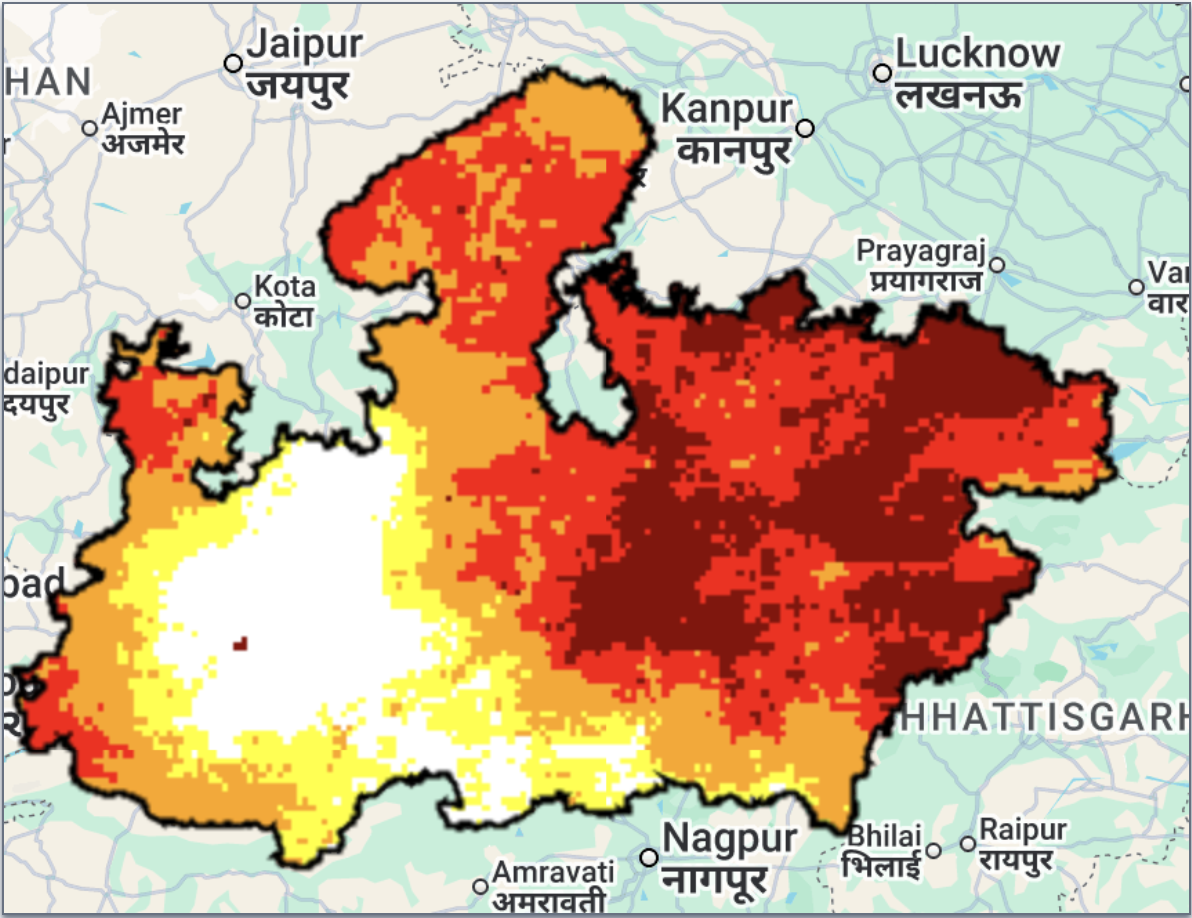
\includegraphics[width=\textwidth]{spei_annual_2015.png}
        \caption{SPEI-12 for the full year 2015, confirming severe annual drought.}
        \label{fig:2015_annual}
    \end{subfigure}
    \caption{Multi-scalar SPEI analysis for the 2015 drought event in Madhya Pradesh.}
    \label{fig:2015_results}
\end{figure}

\clearpage % This command ensures all figures are placed before the next section

\section{References}
\printbibliography

\vspace{1cm}
\noindent \textbf{NOTE:} The SPEI-12 here is measured for the calendar year. This can be changed to an agricultural year as per requirements.

\vfill % This command pushes the following content to the bottom of the page

\begin{flushleft}
\hrule
\vspace{0.5cm}
\noindent This pipeline was developed and implemented by: \\
\textbf{Pushkin Mangla} \\
\textit{B.Tech-M.Tech Dual Degree Student} \\
\textit{Department of Computer Science and Engineering, Class of 2029} \\
\textit{Indian Institute of Technology Delhi}
\vspace{0.5cm}

\noindent Under the academic supervision of: \\
\textbf{Prof. Aaditeshwar Seth} \\
\textit{Department of Computer Science and Engineering} \\
\textit{Indian Institute of Technology Delhi}
\end{flushleft}

\end{document}
